% !TEX Program = xelatex

%\documentclass[12pt]{article}
\documentclass[12pt]{ctexart}

\input{/home/drh/Templates/latex/preamble-ch.tex}

\begin{document}

\setmainfont{Times New Roman}[
 	UprightFeatures= {
		Scale=MatchLowercase,
		Scale=1.08,
 		OpticalSize=14
 	}
]
\setlength{\baselineskip}{22pt}
\pagestyle{empty}


\ 

{
\vspace{50pt}
\centering\fontsize{24pt}{\baselineskip}\textbf{第三届“通达杯”ADI软件无线电大赛}

\vspace{30pt}
\centering\fontsize{36pt}{\baselineskip}\textbf{项目报告}

}

\vspace{170pt}
\begin{table}[htbp]
	\centering
	\fontsize{14pt}{\baselineskip}\songti
\begin{tabular}{ll}
	团队名称:\quad  &\underline{\qquad 我说的都队\hspace{1.97cm} } \bigskip \\
	所在学校:\quad  &\underline{\qquad 华中科技大学\hspace{1.48cm} } \bigskip \\
	所在学院:\quad  &\underline{\qquad 电信学院\hspace{2.462cm} } \bigskip \\
	队长姓名:\quad  &\underline{\qquad 卢玮\hspace{3.444cm} } \bigskip \\
	队长邮箱:\quad  &\underline{\qquad 2326521374@qq.com\hspace{0.375cm} } \bigskip \\
	队员姓名:\quad  &\underline{\qquad 董瑞华,李瑞源 \hspace{0.87cm} } \bigskip \\
	指导教师:\quad  &\underline{\qquad 黑晓军\hspace{2.953cm} } \bigskip \\
\end{tabular}
\end{table}
\newpage
\pagestyle{plain}



\section{所选题目}
\noindent \fontsize{14pt}{\baselineskip}\textbf{题目一\quad 跳频通信}

\noindent \textbf{内容:}

利用pluto实现无线跳频通信。

\bigskip
\noindent \textbf{要求:}

 在中心频率433.920(430.050$\sim$434.790MHz),以200kHZ为带宽,在两台pluto之
 间通过无线跳频(跳频频率不小于4个)传输文字或语音信息。
 
\bigskip
\noindent \textbf{传输内容:}

 文本大小:不小于2Kbit,需要选手连续发生10次,接收端计算误比特率,小于
 1\%为有效传输距离,可以使用信道编码。

 基础要求:传输文本 

 提高要求:传输语音
 
\bigskip
\noindent \textbf{跳频方式:}

 基础要求:顺序跳频

 提高要求:随机跳频 
 
\bigskip
\noindent \textbf{通信距离:}

基础要求:通信距离2米以内

提高要求:通信距离2米以上 

\bigskip
\noindent \textbf{误码率:}

基本要求:<1\%

提高要求:<0.01\% 

\bigskip
\noindent \textbf{调制方式:}

基础要求:FM

提高要求:MSK/GFSK/BPSK/QPSK/OFDM



\section{系统方案}

\subsection{整体方案}

本方案中,跳频事件必须由发送方(A机)发起,接收方(B机)按A机要求完成跳频
后,需要向A机发送确认信号。A机在发起跳频请求后、收到B机确认信号前,不应
该再向B机发送任何其他信号(因为此时无法确认B机在哪个频段)。

通信时,发送方(A机)和接收方(B机)有相同的初始频率和相同的跳频序列。A机在
数据载荷前加上控制字段,用BPSK调制,传输到B机。B机根据控制字段选择接收数
据,或者跳频并返回ACK确认信号。

\subsection{数据包格式}

在进行BPSK调制前,每个包的原始数据的长度为64字节,如图\ref{pack-struc}所示。数据包各字段的作用为:
\begin{figure}[htbp]
	\centering
	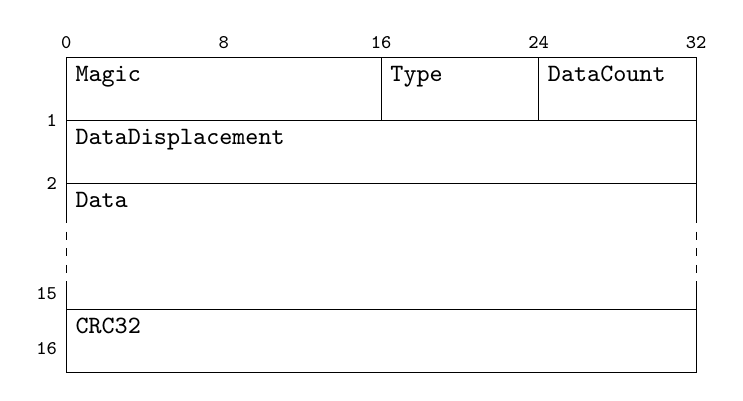
\begin{tikzpicture}
		\tt\small
%  		\draw[gray!40] (0,-5) grid (10,0);
		\draw (0,0) node[above]{\scriptsize 0} 
			(2,0) node[above]{\scriptsize  8}
			(4,0) node[above]{\scriptsize  16}
			(6,0) node[above]{\scriptsize  24}
			(8,0) node[above]{\scriptsize  32};
		\draw (0,-0.8) node[left]{\scriptsize  1}
			(0,-1.6) node[left]{\scriptsize  2}
			(0,-3) node[left]{\scriptsize  15}
			(0,-3.7) node[left]{\scriptsize  16};

		\draw (0,-0.8) -- (0,0) node[below right]{Magic} -- (4,0) -- (4,-0.8);
		\draw (4,0) node[below right]{Type} -- (6,0) -- (6,-0.8);
		\draw (6,0) node[below right]{DataCount} -- (8,0) -- (8,-0.8);

		\draw (0,-1.6) -- (0,-0.8) node[below right]{DataDisplacement} 
			-- (8,-0.8) -- (8,-1.6);

		\draw (0,-2.0) -- (0,-1.6) node[below right]{Data} 
			-- (8,-1.6) -- (8,-2.0);
		\draw[dashed] (0,-2.0) -- (0,-2.9)
			(8,-2.0) -- (8,-2.9);
		\draw (0,-2.9) -- (0,-3.2) -- (8,-3.2) -- (8,-2.9);

		\draw (0,-3.2) node[below right]{CRC32} -- (0,-4)
			-- (8,-4) -- (8,-3.2);
	\end{tikzpicture}
	\caption{数据包结构}
	\label{pack-struc}
\end{figure}

\begin{enumerate}
	\item[(1) ] Magic:\ 2个字节,依次为0xad和0x13,表示该数据包满足图\ref{pack-struc}所示的结构,可以被进一步解析。
	\item[(2) ] Type:\ 1个字节,表示数据包的类型,其值可以为:
	\begin{enumerate}
		\item 0x0:\ Hopping SYN(跳频同步),通知接收方(B机)跳至下一个频率。
		\item 0x1:\ Hopping ACK(跳频确认),通知发送方(A机)跳频已完成。
		\item 0x2:\ File,用于发起一次文件传输,文件长度作为Data。B机收到后,应该打开一个新的文件,并向A机回复一个同类型的数据包,表示接收成功。
		\item 0x3:\ File Secondary,用于发送实际文件内容,B机收到后,应该回复一个同类数据包。
	\end{enumerate}
	\item[(3) ] DataCount:\ 仅当Type为0x2和0x3时有效。1个字节,表示数据段中,有效数据的
	长度(以字节为单位)。
	\item[(4) ] Data:\ 56字节的数据段,仅当Type为0x2和0x3时有效。
		\begin{enumerate}
			\item 当Type为0x2时,Data段有效数据为uint32类型的TotalDataCount,用于向B机告知待传文件的总大小。
			\item 当Type为0x3时,从Data段开始的DataCount字节为有效数据载荷。
		\end{enumerate}
	\item[(5) ] CRC32:\ 32位CRC校验,用于验证接收到的数据是否存在差错。
\end{enumerate}


\subsection{发送流程图}
	发送方(A机)的通信流程如图\ref{send-routine}所示。
\begin{figure}[htbp]
	\centering
 	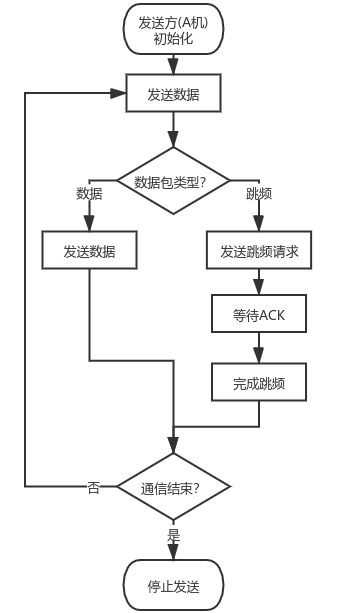
\includegraphics[scale=0.6]{../figures/send-routine.png}
	\caption{发送流程图}
	\label{send-routine}
\end{figure}

\subsection{接收流程图}
	接收方(B机)的通信流程如图\ref{rcv-routine}所示。
\begin{figure}[htbp]
	\centering
 	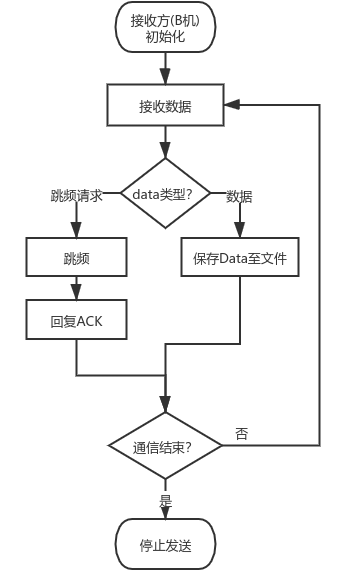
\includegraphics[scale=0.6]{../figures/rcv-routine.png}
	\caption{接收流程图}
	\label{rcv-routine}
\end{figure}


\section{系统理论分析和计算}

\subsection{BPSK调制原理}

	在二进制数字调制中,用已调信号载波$S(t)$的相位$\varphi_c$表示二进制信号$x(t)$,称为
二进制移相键控(BPSK, Binary Phase Shift Keying)。
$\varphi_c = 0$表示$x(t)$为$0$,$\varphi_c = \pi$表示$x(t)$为$1$,因此有:
\begin{align}
	S(t) = \cos[\omega_c t + \pi \cdot x(t)]
	\label{eq-1}
\end{align}

\noindent 其中$\omega_c$为载波频率。令调制系数:
\begin{align}
	m(t) = 
	\left\{\begin{aligned}
		& 1, & x(t) = 0 \\
		−&1, & x(t) = 1
	\end{aligned}\right.
	\label{eq-2}
\end{align}

\noindent 将\eqref{eq-2}代入\eqref{eq-1}式,可得:
\begin{align}
	S(t) = m(t) \cdot \cos(\omega_c t)
	\label{eq-3}
\end{align}

	结合上述分析,BPSK调制模型如图\ref{mod-prin}所示,调制信号波形如图\ref{mod-exp}所示。由于BPSK调制不使用$Q(t)$,图\ref{mod-exp}中$Q(t)$路始终为$0$。

\begin{figure}[htbp]
	\centering
 	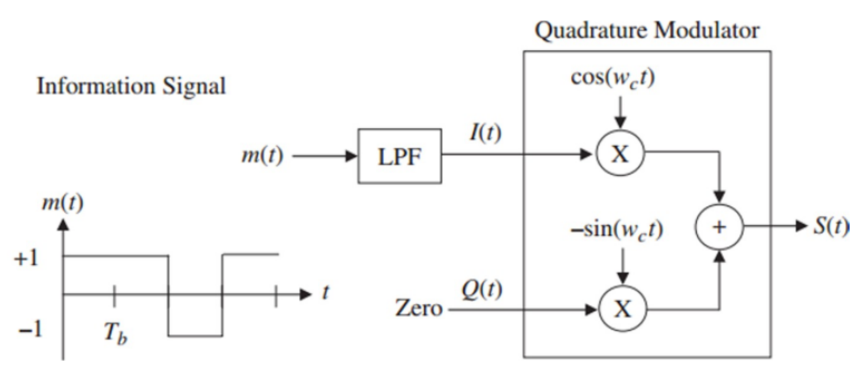
\includegraphics[scale=0.5]{../figures/mod-prin.png}
	\caption{BPSK调制原理图}
	\label{mod-prin}
\end{figure}

\begin{figure}[htbp]
	\centering
 	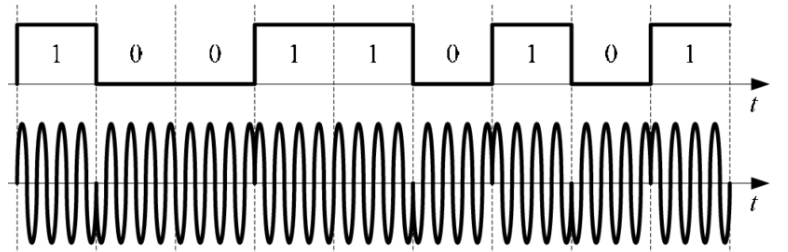
\includegraphics[scale=0.5]{../figures/mod-exp.png}
	\caption{BPSK调制信号示例}
	\label{mod-exp}
\end{figure}

\subsection{BPSK解调原理}
	BPSK信号通常采用相干解调,且需要使用与发送方BPSK信号同频同相的相干载
波,即$\cos(\omega_c t)$。由\eqref{eq-3}式和$\cos(\omega_c t)$的性质可知,
从$S(t)$中还原$m(t)$的一种方法为:
\begin{align}
	\hat m(t) = 
	\frac{2}{T} \int_0^{T_c} S(\tau − t) \cos(\omega_c \tau) d\tau
	\label{eq-4}
\end{align}

	由\eqref{eq-2}式,$m(t)$可化为:
\begin{align}
	m(t) = 2x(t) - 1
	\label{eq-5}
\end{align}

	联立\eqref{eq-4}、\eqref{eq-5}两式可得:
\begin{align}
	\hat x(t) = 
	\frac{1}{2} + 
	\frac{1}{T} \int_0^{T_c} S(\tau − t) \cos(\omega_c \tau) d\tau
	\label{eq-6}
\end{align}

	若使用正弦波进行调制和解调,则有:
\begin{align}
	\hat x(t) = 
	\frac{1}{2} + 
	\frac{1}{T} \int_0^{T_c} S(\tau − t) \sin(\omega_c \tau) d\tau
	\label{eq-7}
\end{align}

	结合上述分析,BPSK相干解调流程和相应的波形,分别如图\ref{dmod-prin}、图\ref{dmod-exp}所示:
\begin{figure}[htbp]
	\centering
 	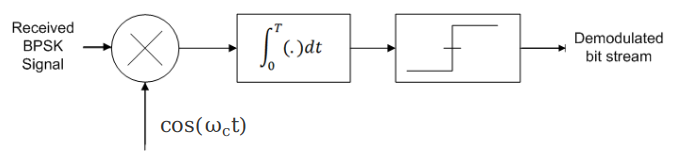
\includegraphics[scale=0.65]{../figures/dmod-prin.png}
	\caption{BPSK相干解调}
	\label{dmod-prin}
\end{figure}


\begin{figure}[htbp]
	\centering
 	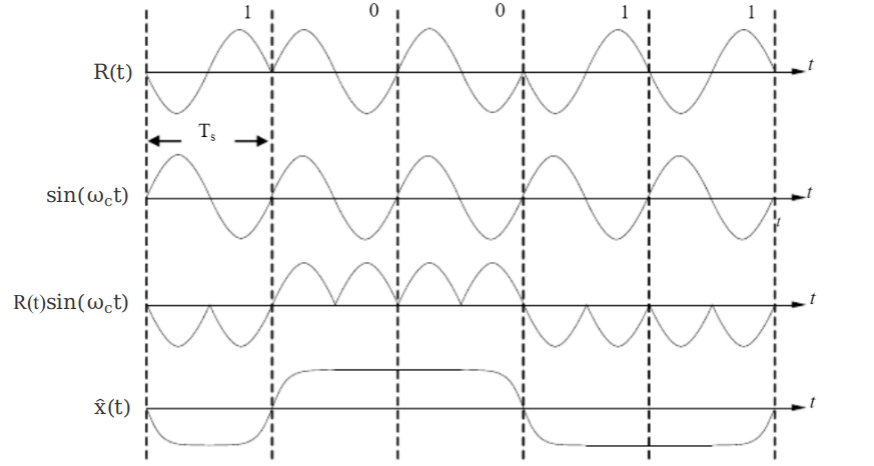
\includegraphics[scale=0.6]{../figures/dmod-exp.png}
	\caption{BPSK解调波形}
	\label{dmod-exp}
\end{figure}


\subsection{跳频通信的基本原理}

	跳频通信是扩频通信的一种方式,是指载波频率在比较宽的频带范围内根据某种图
案(序列)进行跳变的通信方式,基本原理如下:
\begin{figure}[htbp]
	\centering
 	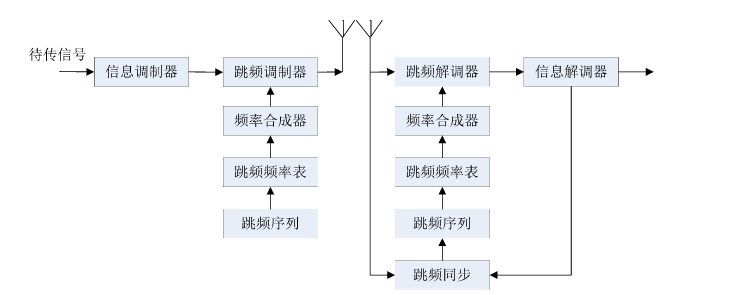
\includegraphics[scale=0.65]{../figures/hop-prin.png}
	\caption{跳频通信原理}
	\label{hop-prin}
\end{figure}

	在发射端,待传数字信号经过调制,形成带宽为$W_1$的基带信号;随后通过伪随机
码发生器得到跳频序列,使用该序列选择跳频频率表中的对应频率,控制发端频率合成
器产生不断跳变的载波。将基带信号和跳频载波进行调制,得到频率不断跳变的射频信
号,即跳频信号。跳频信号在在带宽为$W_2$的频带范围内随机跳变($W_2>>W_1$),系统实
现了从窄带带宽$W_1$到跳频信号使用带宽$W_2$的频谱扩展。在接收端,通过同步模块使
得收端频率合成器产生的跳变规律相同的本地载波,实现相干解调。

	同步模块中,常用的跳频同步方法有外时钟法和自同步法。本方案采用了更简易的
方法:由发送方发起同步要求,接收方随后跳频并回复确认信号,发送方在收到确认之
后才跳频。这种阻塞式的跳频虽然性能较差,且要求双工通信,但实现起来更简单,同
时也能满足基本的跳频通信要求。

\section{跳频演示}
为便于演示跳频效果,我们让发送方(A机)向接收方(B机)重复发送相同的数据包,
并让A机用第15个包向B发送跳频请求。则跳频前、B跳频完成且A仍在等待、A和
B都完成跳频时的结果如图\ref{hop-a0b0}、\ref{hop-a0b1}、\ref{hop-a1b1}所示:

\begin{figure}[htbp]
	\centering
 	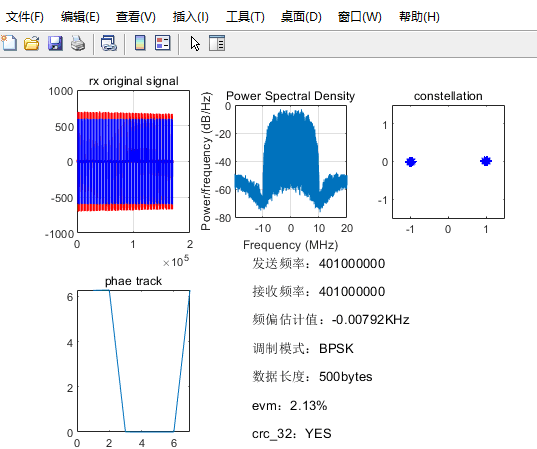
\includegraphics[scale=0.6]{../figures/hop-a0b0.png}
	\caption{跳频前}
	\label{hop-a0b0}
\end{figure}

\begin{figure}[htbp]
	\centering
 	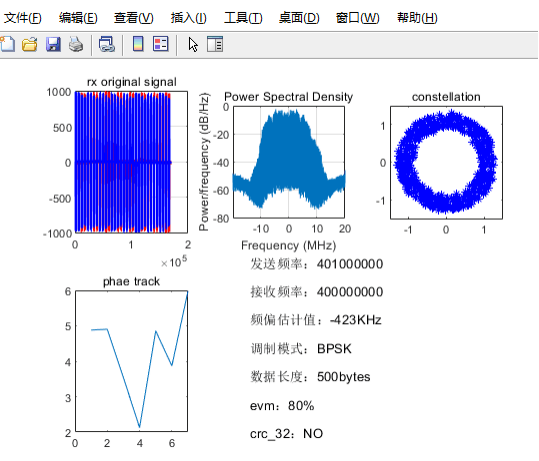
\includegraphics[scale=0.6]{../figures/hop-a0b1.png}
	\caption{B已跳频且A未跳频}
	\label{hop-a0b1}
\end{figure}

\begin{figure}[htbp]
	\centering
 	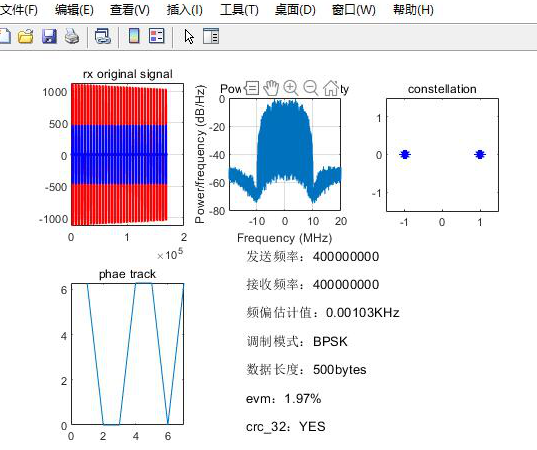
\includegraphics[scale=0.6]{../figures/hop-a1b1.png}
	\caption{A和B都完成跳频}
	\label{hop-a1b1}
\end{figure}


\section{结论}

	现阶段,我们已实现了下列功能:
\begin{enumerate}
	\item 成功传输文本(TXT格式)和语音(WAV格式);
	\item 跳频个数为5个,且跳频序列伪随机;
	\item 通信距离最大为0.7m;
	\item 误码率在0.3\%$\sim$0.9\%之间;
	\item 调试方式为BPSK。
\end{enumerate}


\section{参考文献}

\noindent [1]张辉,曹丽娜. 现代通信原理与技术. 西安电子科技大学出版社.
 
\noindent [2]高西全,丁玉美. 数字信号处理. 西安电子科技大学出版社.
 
\noindent [3]王玉磊. 从零开始学MATLAB. 中国铁道出版社.

\end{document}

